\documentclass[
%  draft,
  10pt,
  a4paper,
  parskip,
  titlepage,
%  twocolumn,
%  twoside,
%  openright,
%  listof=totocnumbered,
%  bibliography=totocnumbered,		% Literaturverzeichnis im Inhaltsverzeichnis aufführen und nummerieren
%  liststotoc,				% Verzeichnisse im Inhaltsverzeichnis aufführen
%  idxtotoc				% Index im Inhaltsverzeichnis aufführen
]{scrartcl}
%]{report}
%]{scrbook}

\usepackage{graphics}
\usepackage{epstopdf}
\usepackage[utf8]{inputenc}
\usepackage[english]{babel}
\usepackage{csquotes}
\usepackage{amsmath}
\usepackage{amsfonts}
\usepackage{rotating}
\usepackage{float}
\usepackage{amssymb}
\usepackage[svgnames]{xcolor}
\usepackage{tikz}
\usepackage{listings}
\usepackage[breaklinks]{hyperref}
\usepackage[all]{hypcap}        % jump to the start of table/figure instead to the caption of it (fix for hyperref)
%\usepackage{url}
\usepackage{placeins}           % for \FloatBarrier
\usetikzlibrary{arrows,positioning,shapes} 
\usepackage{titlepage}
\usepackage{textcomp} % for \textgreater and \textless
\usepackage{comment}
\usepackage{caption}
\usepackage{subcaption}
\usepackage{xcolor}
\usepackage{chngpage}
\usepackage{multirow}

\usepackage{fancyhdr}
\pagestyle{fancy}
\fancyhead[LO,RE]{\iffloatpage{}{Report: Analysis of a Messaging System}}
\fancyhead[RO,LE]{\iffloatpage{}{\thepage}}
\fancyfoot{}
\renewcommand{\headrulewidth}{\iffloatpage{0pt}{0.4pt}}

\lstset{ %
  basicstyle=\footnotesize,       % the size of the fonts that are used for the code
  numbers=left,                   % where to put the line-numbers
  numberstyle=\tiny\color{gray},  % the style that is used for the line-numbers
  numbersep=5pt,                  % how far the line-numbers are from the code
  backgroundcolor=\color{white},  % choose the background color. You must add \usepackage{color}
  showspaces=false,               % show spaces adding particular underscores
  showstringspaces=false,         % underline spaces within strings
  showtabs=false,                 % show tabs within strings adding particular underscores
  frame=single,                   % adds a frame around the code
  rulecolor=\color{black},        % if not set, the frame-color may be changed on line-breaks within not-black text (e.g. commens (green here))
  tabsize=2,                      % sets default tabsize to 2 spaces
  captionpos=b,                   % sets the caption-position to bottom
  breaklines=true,                % sets automatic line breaking
  breakatwhitespace=false,        % sets if automatic breaks should only happen at whitespace
  escapeinside={\%*}{*)},         % if you want to add a comment within your code
  morekeywords={*,...}            % if you want to add more keywords to the set
}


\setcounter{tocdepth}{5}   
\setcounter{secnumdepth}{5} 

\author{Thomas Frick (LEGI)\\Matthias Ganz (04-862-850)\\Philipp Rohr (04-397-030)}

\makeatletter
\AtBeginDocument{\markboth{\@author}{\@title}}   % gives access to those variables through \@author

\title{Implementation of a Virtual File System}
\date{\today}

\hypersetup
{
  pdftitle={\@title},
  pdfauthor={\@author},
  pdfsubject={}
}

\clubpenalty=10000
\widowpenalty=10000\displaywidowpenalty=10000 

\newcommand{\code}[1]{\texttt{#1}}
\newcommand{\console}[1]{\fbox{\texttt{#1}}}
\newcommand{\file}[1]{\textsl{#1}}

\newcommand{\anmerkung}[1]{\marginpar{\color{red}\footnotesize{#1}}}
\newcommand{\todo}[1]{{\color{red}#1\index{todo!#1}}\anmerkung{{\color{red} todo}}}



\setcounter{tocdepth}{2}
\begin{document}
\maketitle

\tikzstyle{app}=[anchor=center,minimum width=3 cm,minimum height=2 cm,rectangle,rounded corners,draw=black, top color=white, bottom color=blue!30,very thick, text centered]
\tikzstyle{map}=[anchor=center,minimum width=1 cm,minimum height=1 cm,rectangle,rounded corners,very thick, text centered,draw=black,fill=white]
\tikzstyle{event}=[map, fill=green!30,very thick, text centered]
\tikzstyle{arrow}=[->,thick]
\tikzstyle{derive}=[->, >=open triangle 90, thick]

\tikzstyle{use}=[<-, >=open diamond, thick]
\tikzstyle{need}=[<-, >=diamond, thick]

\tikzstyle{Interface}=[rectangle,draw=black, fill=yellow!60,rotate=90]
\tikzstyle{file}=[anchor=center,draw=black, top color=white, bottom color=yellow!30,thick, text centered]

\tikzstyle{class}=[anchor=center,draw=black, fill=yellow!30, thick, rectangle split, rounded corners, rectangle split parts=3, align=left]

\tikzstyle{page}=[anchor=center,minimum width=1 cm,minimum height=1 cm,rectangle, thick, text centered,draw=black,fill=white]
\tikzstyle{label}=[anchor=center,text centered]

\tikzstyle{physical}=[fill=yellow!30]
\tikzstyle{virtual}=[fill=blue!60]
\tikzstyle{org}=[fill=blue!10]



\setcounter{secnumdepth}{3}
\setcounter{tocdepth}{3}
\tableofcontents

\begin{abstract}
\section*{Abstract}
The \textit{Virtual File System} was implemented during the course
\textit{Java and C\# in depth}.

This version of the document describes the project at the final state of
milestone 1. and so on\ldots
 
\end{abstract}


\section{The Full Model}
After we did one more experiment that is explained in the appendix
 I could could examine the measured values and made some observations that are
  described in this section. Based on those observations I built the full model
   that will be the basis of a mean value analysis shown further in the document.

\subsection{Definitions}
blablab

\subsection{Observations}
This is a table (table \ref{table:measuredData}) measured throughout the
 and a footnote \footnote{Described in the appendix \ref{sec:client_scale_out}} 
 
\begin{table}[h!]
 \centering
 \begin{tabular}{| r| rrrr | rr | r |}
    \hline \textbf{$N$} & \textbf{$R_{puts}$} & \textbf{$R_{retrieves}$} & \textbf{$R_{meas}$} & \textbf{$X_{meas}$} & \textbf{$X_{calc}$} & \textbf{$R_{calc}$}  & \textbf{$Z_{calc}$} \\
    \hline 32  & 69  & 112 & 181 & 176.5 & 176.8 & 181 & 0 \\
    \hline 64  & 72  & 113 & 185 & 344.7 & 345.9 & 186 & 1 \\
    \hline 96  & 81  & 115 & 196 & 486.4 & 489.8 & 197 & 1 \\
    \hline 128 & 98  & 119 & 217 & 586.8 & 589.9 & 218 & 1 \\
    \hline 160 & 124 & 130 & 254 & 628.3 & 629.9 & 255 & 1 \\
    \hline 192 & 161 & 156 & 317 & 603.9 & 605.7 & 318 & 1 \\
    \hline 224 & 213 & 204 & 417 & 536.4 & 537.2 & 418 & 1 \\
    \hline 256 & 251 & 230 & 481 & 531.2 & 532.2 & 482 & 1 \\ 
    \hline
 \end{tabular}
\caption{Measured (on client side) and calculated data of the whole system.}
\label{table:measuredData}
\end{table}


\subsection{The Model}
and a figure \ref{fig:full_model}.  fancy foobar

\begin{figure}[h!]
\centering
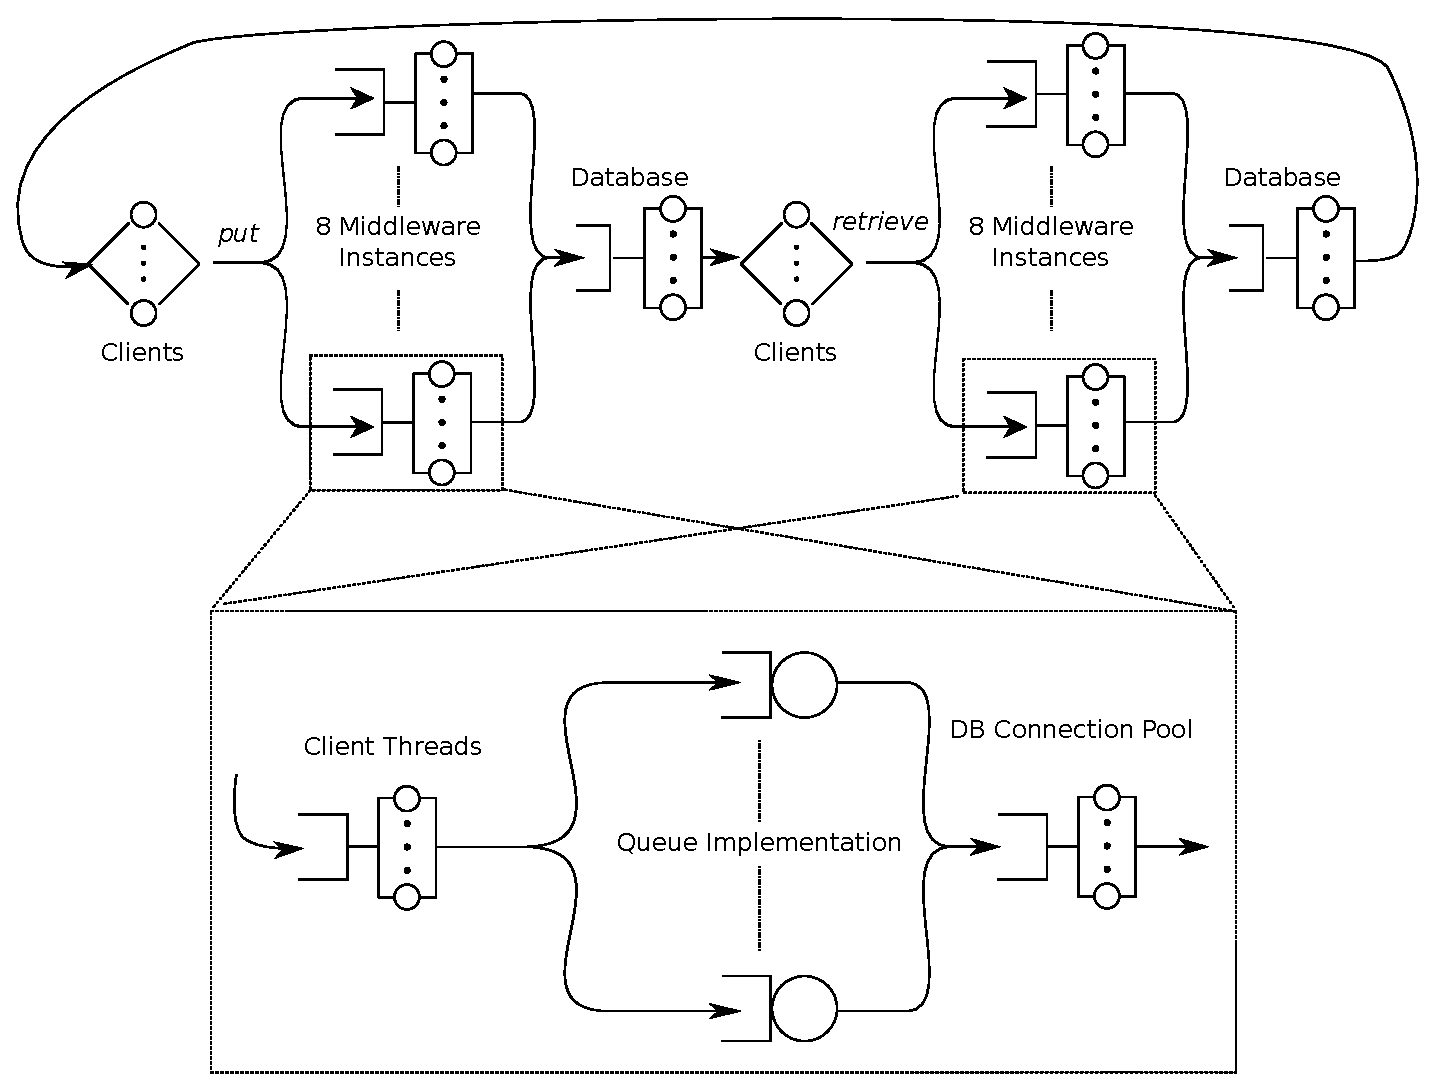
\includegraphics[width=1\textwidth]{figures/full_model.eps}
\caption{Full model of the system.}
\label{fig:full_model}
\end{figure}

\newpage

citation\cite{Raj}. 

some math

\[\mu(n) =
\left\{
	\begin{array}{ll}
		n/S  & \mbox{if } n=1,2,...,m-1 \\
		m/S & \mbox{if } n=m,m+1,...,\infty
	\end{array}
\right.
 \]




\subsection{The \emph{real} implemenation}

Eventually some code that handles a virtual disk was developed and is described
in this section.

\subsubsection{The File Format}


This section describes the binary file format used by the file system inside a
virtual disk.
The file is separated into three major parts. The header, index and the data
section. Each of them is described below.

\begin{figure}[h!]
\centering
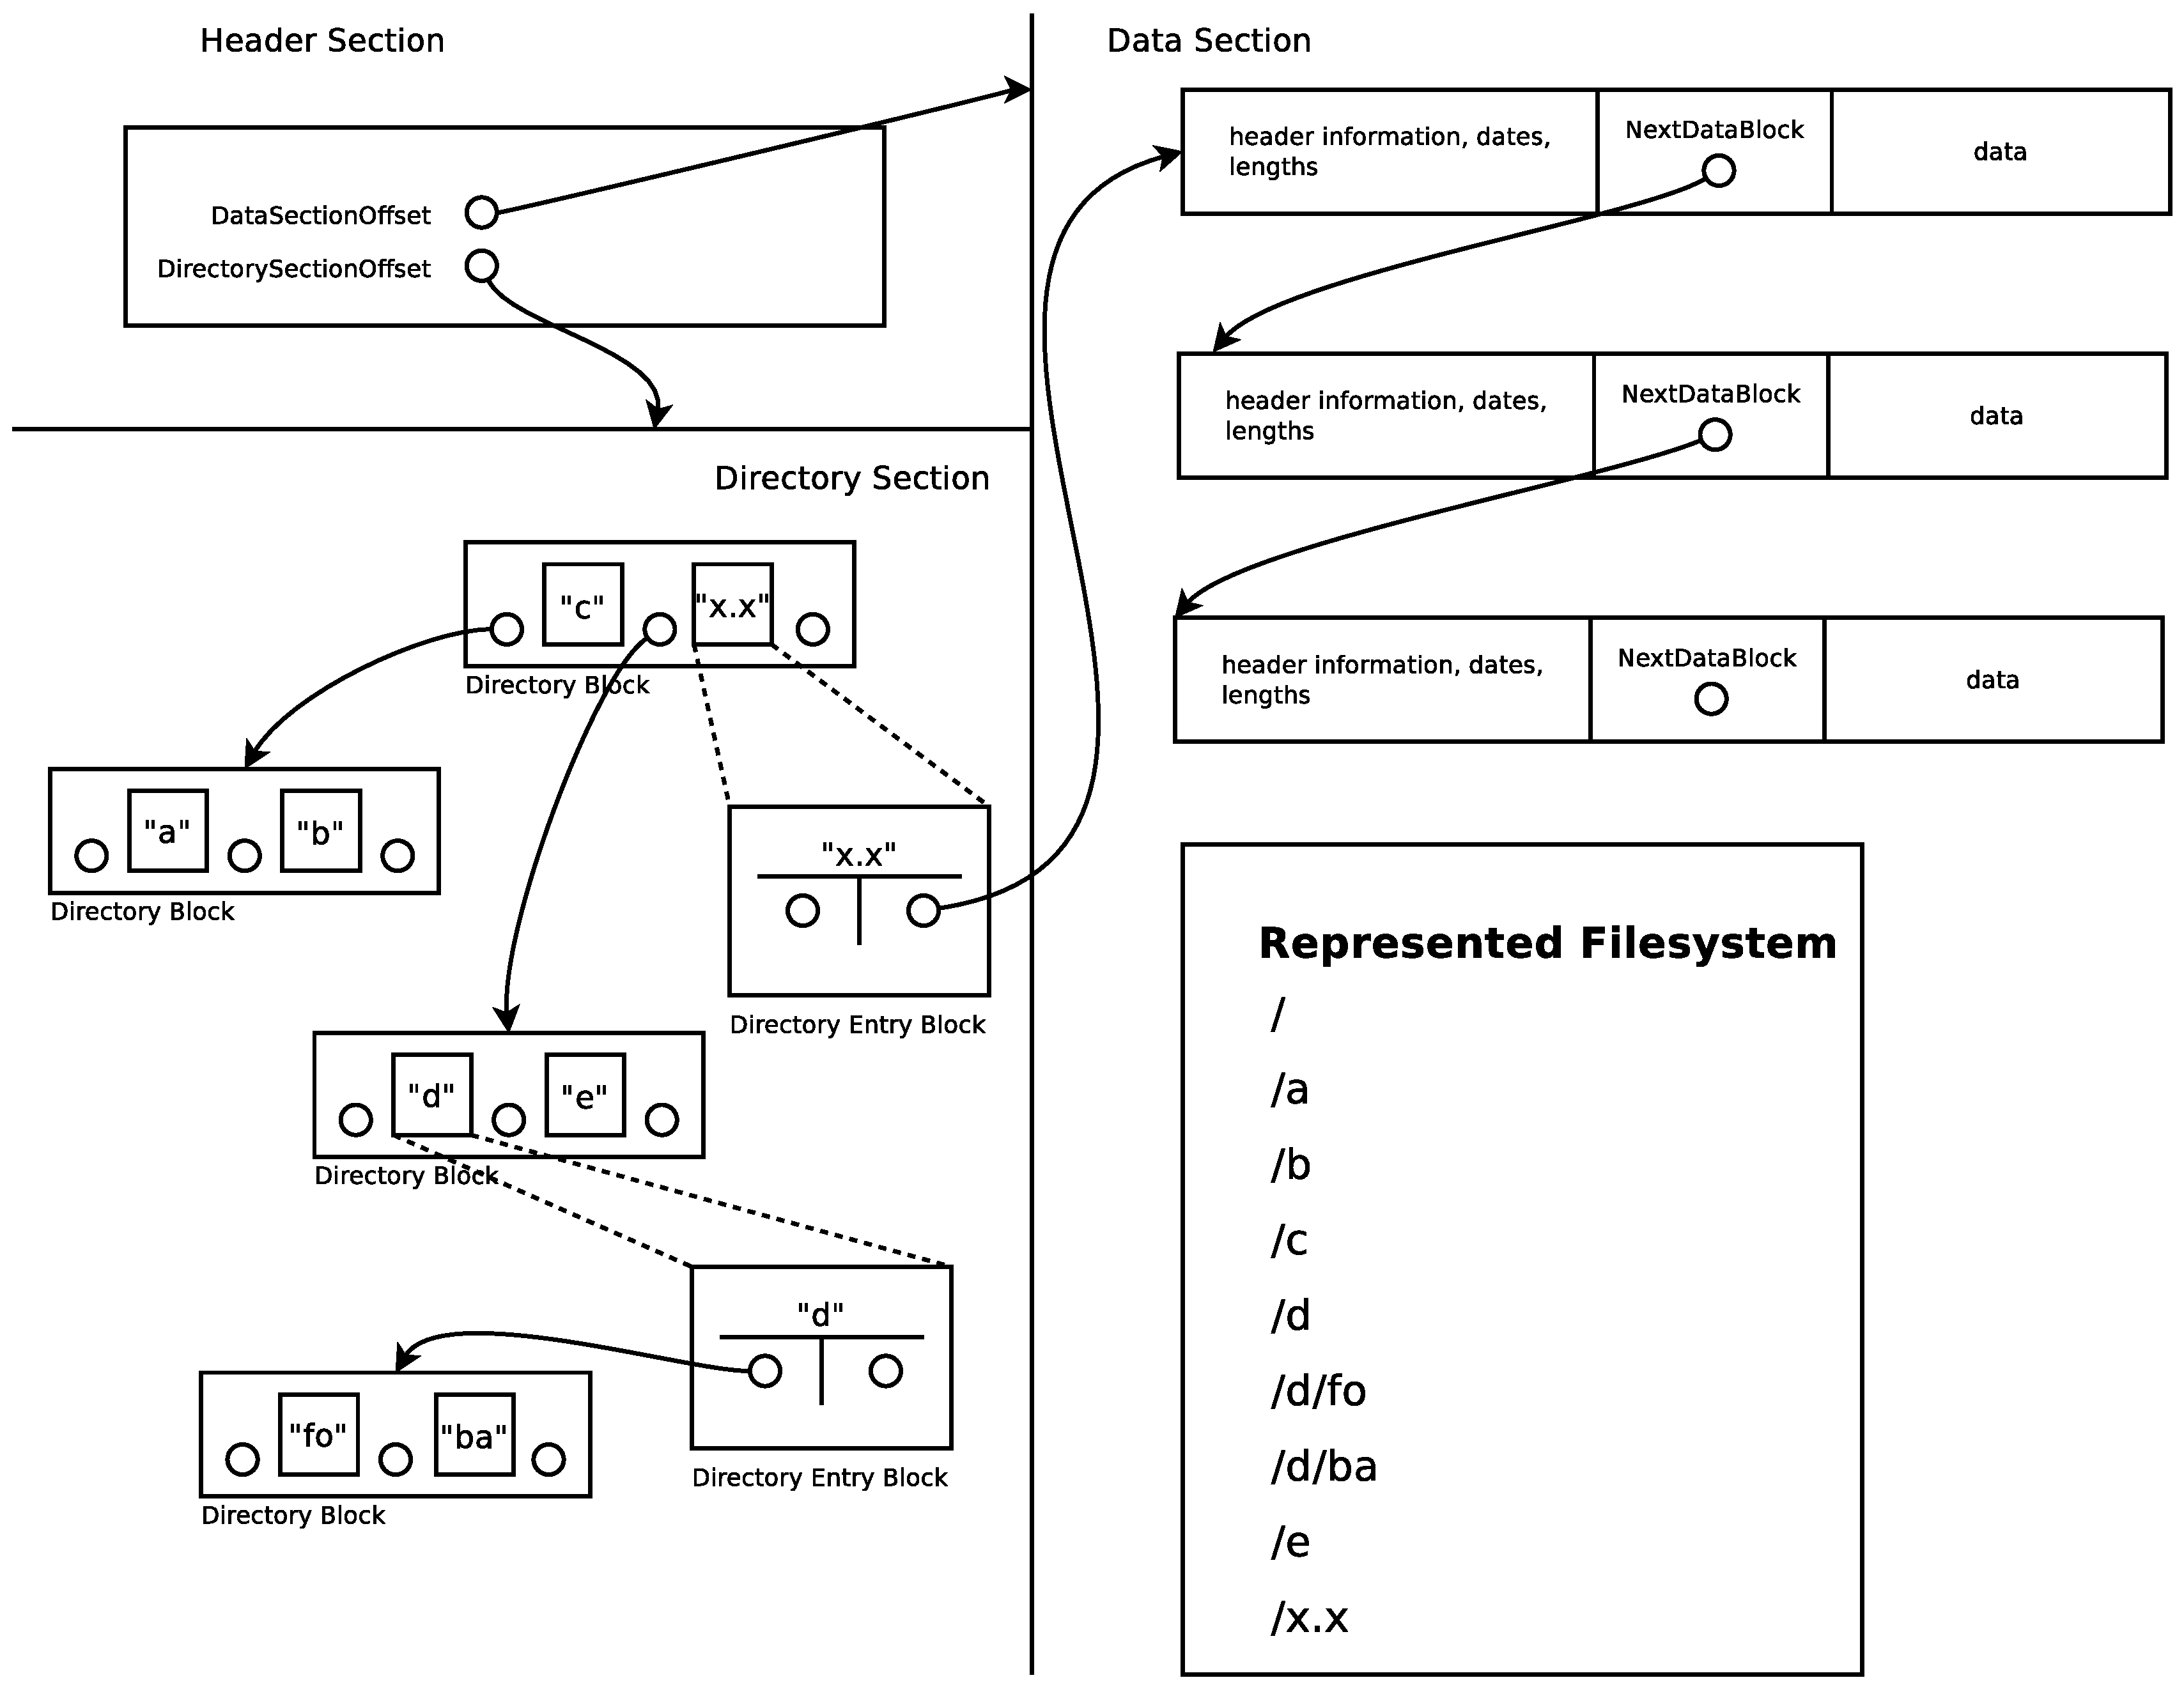
\includegraphics[width=1\textwidth]{figures/fileFormat.eps}
\caption{Overview of a disk}
\label{fig:disk_overview}
\end{figure}

\paragraph{Header Section} The header section contains some general information
about the currently opened virtual disk. The details can be found in the
following table:

\begin{tabular}{|l|l|p{5cm}|}
\hline
  \textbf{Name} & \textbf{Length} & \textbf{Description}
\\  \hline
  Info & 50 byte UTF-8 String & Contains something like Badger VFS 2013 V1.0 
\\ \hline
  Version & 10 byte UTF-8 String & Contains something like "1.0"
\\ \hline
  Compression used & 20 byte UTF-8 String & null or indicates compression used for this file
\\ \hline
  Encryption used & 20 byte UTF-8 String & null or indicates encryption used for this file
\\ \hline
 DirectorySectionOffset & long (8 byte) &  File offset where our directory section
 starts \\ \hline
 DataSectionOffset & long (8 byte) &  File offset where our data section starts
\\ \hline
 SaltString & 8 bytes  & Salt used to hash username and password randomly string generated while creating this
   file
 \\ \hline
  Password & xxx bytes  & CryptoHash (SHA-whatever) of Password+SaltString
\\ \hline

\end{tabular}


\paragraph{Directory Section}

The directory section describes which files and folders belong to which parent directory. This section has a fixed size and contains so called DirectoryBlocks which also have a fixed size. This makes management an manipulation easy. To each directory belongs a B-Tree structure which lists all contained entries.


\subparagraph*{Directory Block}

One Directory Block represents a Node in our B-Tree of order 2.

\begin{tabular}{|l|l|p{5cm}|}
\hline
  \textbf{Name} & \textbf{Length} & \textbf{Description}
\\  \hline

DirectoryHeader & 1 byte & Header information. This header makes it easy to determine whether a DirecotryBlock is in used or not (memory management)

\\  \hline

DirectoryEntryBlock1 & 128 byte & The smaller key inserted into our B-Tree

\\  \hline

DirectoryEntryBlock2 & 128 byte & The bigger key inserted into our B-Tree

\\  \hline

DirectoryBlockLink1 & 8 byte & Points to another DirectoryBlock which contains keys smaller than DirectoryEntryBlock1

\\  \hline

DirectoryBlockLink2 & 8 byte & Points to another DirectoryBlock which contains keys bigger than DirectoryEntryBlock1 but smaller than DirectoryEntryBlock2

\\  \hline

DirectoryBlockLink3 & 8 byte & Points to another DirectoryBlock which contains keys bigger than DirectoryEntryBlock2

\\  \hline


\end{tabular}

\subparagraph*{Directory Entry Block}

Represents a single directory or file.

\begin{tabular}{|l|l|p{5cm}|}
\hline
  \textbf{Name} & \textbf{Length} & \textbf{Description}
\\  \hline

Filename & 112 byte & UTF-8 Filename String 


\\  \hline

DataBlockLocation & 8 byte & Pointer to a DataBlock located in the Data Section.
This DataBlock holds some meta information about the current directory


\\  \hline

DirectoryEntryTreeRoot & 8 bytes & Pointer to a DirectoryBlock located in the
Directory Section. This referenced DirectoryBlock is the Root Block of a B-Tree
containing all entries of that directory specified by the current Directory Entry Block.
\newline

\textbf{This field containing a 0 indicates that this entry is a file not a directory}



\\  \hline

\end{tabular}


\paragraph{Data Section}
The data section is split into blocks where each of them is X bytes long.
Each block contains some amount of data and points to a subsequent block


Block layout \\

\begin{tabular}{|l|l|p{5cm}|}
\hline
  \textbf{Name} & \textbf{Length} & \textbf{Description}
\\  \hline
 BlockHeader & 1 byte & 
 \\
 \hspace{0.2cm} 0) Header-Bit (LSB) & &  If set to 1 this is the first datablock
 of a file.
 \\ 
 \hspace{0.2cm} 1) not used & &  
 \\ 
 \hspace{0.2cm} 2) not used & &  
 \\ 
 \hspace{0.2cm} 3) not used & &  
 \\ 
 \hspace{0.2cm} 4) not used & &  
 \\ 
 \hspace{0.2cm} 5) not used & &  
 \\ 
 \hspace{0.2cm} 6) not used & &  
 \\ 
 \hspace{0.2cm} 7) not used & &  
 
\\  \hline
 NextDataBlock & 8 byte & 
 Points to the start address of the next Datablock (linked list).
    0 if this is the last DataBlock of a certain file or folder.
\\  \hline
  CreationDate & 8 byte & UTC Time when this file was created
  \newline \textit{This field only exists if Header-Bit is set to 1}
\\  \hline

  DataLength & 4 byte &
    Indicates the number of data saved on this DataBlock.
    
\\  \hline
 Data & n byte & user data (may be encrypted/compressed)
\\  \hline
\end{tabular}


\paragraph{The root directory}


\subsubsection{compression layer}

To reduce the data volume within the virtual disk, compression on each file can
be enabled. Currently available compression algorithms are run length encoding
\cite{rle} and LZ77 \cite{lz77}.

\paragraph{Run Length Encoding}

The available 8bit run length encoding(rle) algorithm is a very simple form of
data compression where multiple occurrence of the same byte were stored as a
single byte value and the corresponding count. It is useful for simple graphic
images like line drawings and icons.

\paragraph{LZ77}

Abraham Lempel and Jacob Ziv introduced the LZ77 lossless compression algorithm
in 1977. Newer compression methods such as GZIP or DEFLATE often use LZ77-based
algorithms. The compression is achieved by replacing the data with a reference
to an earlier existing copy in the data input stream. For that a window of
a certain size is held in memory where existing copies of the current data are
searched.


\appendix
\section{Glossary}

\paragraph{VFS core} The main Java library, that handles all the interaction
with virtual disks and importing/exporting/storing files. It is used by the
command line client and the gui.

\paragraph{Virtual Disk} A virtual disk denotes a container file that is stored
on the host file system. A virtual disk can be opened with the software that is
developed during this project and stores the actual files. The file extension of
the virtual disk is ``*.bfs''.


\section{Command line client}

The command line client allows the usage of the VFS core and is mainly intended
to test the basic functionalities. The console runs either in  management mode
or in filesystem mode. The management mode is entered automatically when
starting the command line client. It allows creating and disposing virtual
disks. The filesystem mode is entered as soon as a virtual disk is opened.

\textbf{TODO: DISCUSSION: sollen ganze ordner importiert und exportiert werden
können? wird dies von der client-seite gehandelt?}

\subsection{startup}
The command line client can be started as follows:

\code{ java -jar VFSCore.jar ch.eth.jcd.badgers.vfs.ui.VFSConsole }

\subsection{commands}
Following commands can be used with the command line client in management mode:

\begin{itemize}
  \item{\textbf{create c:\textbackslash path\textbackslash to\textbackslash
  disk.bfs 1024}} creates virtual disk of size 1024 megabytes on the host
  system
  \item {\textbf{dispose c:\textbackslash path\textbackslash to\textbackslash
  disk.bfs}} deletes the given virtual disk
  \item {\textbf{open c:\textbackslash path\textbackslash to\textbackslash
  disk.bfs}} opens filesystem mode for the given virtual disk
\end{itemize}

follwing commands can be used in filesystem mode:

\begin{itemize}
  \item {\textbf{ls}} lists the contents of the current directory
  \item {\textbf{rm file}} deletes the entry denoted as file
  \item {\textbf{cp src dst}} copies the src file to dst 
  \item {\textbf{import ext\_dst}} imports a ext\_src from the host system to
  dst
  \item {\textbf{export src ext\_src}} exports a src file to the host system
  ext\_dst
\end{itemize}





\listoffigures
\listoftables

\bibliographystyle{plain}
\bibliography{literature}
\end{document}
